\documentclass[11pt,oneside]{article}
\usepackage{geometry}                % See geometry.pdf to learn the layout options. There are lots.
\geometry{letterpaper}                   % ... or a4paper or a5paper or ...
%\geometry{landscape}                % Activate for for rotated page geometry
\usepackage{fullpage}
\usepackage{graphicx}
\usepackage{amssymb}
\usepackage{comment}

%Special formatting packages
%\usepackage{datetime}
%\usepackage{fmtcount}
%\usepackage{timestamp}
\usepackage{fancyhdr}  %fancy headers/footers
\usepackage{pdfpages}  %input pdf pages
\usepackage{everypage} %allow repeating element on each page (for white-out of page numbers)
%\usepackage{tocloft} %table of contents customization
\usepackage{epstopdf}
\usepackage[pdftitle={Rejecta Mathematica Vol. 2, No. 1},pdfauthor={Rejecta Publications, Inc.},pdfsubject={Journal of Mathematical Science},pdfkeywords={journal, rejected paper, math, science, open access},bookmarks=true,colorlinks=true,linkcolor=black,urlcolor=black]{hyperref} %PDF bookmarks and links
%\usepackage{draftcopy} %for Proofs (dvips only)

\DeclareGraphicsRule{.tif}{png}{.png}{`convert #1 `dirname #1`/`basename #1 .tif`.png}

\begin{comment}
%%%%%
% Draft Copy (PDF-latex)
%%%%%
\usepackage{type1cm}
\usepackage{eso-pic}
\usepackage{color}
\makeatletter
\AddToShipoutPicture{%
            \setlength{\@tempdimb}{.5\paperwidth}%
            \setlength{\@tempdimc}{.5\paperheight}%
            \setlength{\unitlength}{1pt}%
            \put(\strip@pt\@tempdimb,\strip@pt\@tempdimc){%
        \makebox(0,0){\rotatebox{45}{\textcolor[gray]{0.75}%
        {\fontsize{6cm}{6cm}\selectfont{DRAFT}}}}%
            }%
}
\makeatother
%%%%%%
% End Draft Copy
%%%%%%
\end{comment}

\pagestyle{fancy}

%Redefine TOC contents title


\begin{document}


%%%%%%%%%%%%%%%%%%%%%%%%%%%%%%%%%%%%%%%%%%%%%%
%Cover Page

%TOC Name
%\renewcommand{\contentsname}{\textsf{Contents}} %new contents title font
\renewcommand{\contentsname}{} %empty contents title

\phantomsection
\addtocontents{toc}{\protect\setcounter{tocdepth}{0}}
\addcontentsline{toc}{section}{\textsf{Rejecta Mathematica Vol. 2, No. 1}}
\addtocontents{toc}{\protect\setcounter{tocdepth}{2}}


%\textheight = 639pt %extend hight of text for this page
%\footskip = 60pt %move down footer for some extra space
\fancyhead{}
\renewcommand{\headrulewidth}{0.0pt}
\fancyfoot{}
%\fancyfoot[C]{2011 Rejecta Publications, Inc.}
\fancyfoot[L]{
\vspace{-1.45cm}
\begin{center}
\footnotesize{2011 Rejecta Publications, Inc.}
\end{center}
\footnotesize{\textsf{This work is published under the Creative Commons Attribution-NonCommercial License.\\
~~~~~~~~~\textbf{License}  \href{http://creativecommons.org/licenses/by-nc/2.5/legalcode}{http://creativecommons.org/licenses/by-nc/2.5/legalcode}\\
~~~~~~~~~\textbf{Human-Readable Summary}  \href{http://creativecommons.org/licenses/by-nc/2.5/}{http://creativecommons.org/licenses/by-nc/2.5/} }}
}
\begin{picture}(0,0)(16,664)  %(width, height)(-x,y) in mm
		\put(0,0){
\includegraphics[width=.048\linewidth]{cc}}
\end{picture}

\begin{center}
 \href{http://math.rejecta.org}{
\includegraphics[width=\linewidth]{logo}}
\end{center}
%\vspace{-.5in}
\vspace{-.53in}
\begin{flushright}
Volume 2, Number 1~|~June 2011\\
{\footnotesize ISSN 1948-8351}\\
\href{http://math.rejecta.org}{\textsf{math.rejecta.org}}\\
\end{flushright}


\hfill
%\vspace{.1in}

\noindent\small{\emph{Rejecta Mathematica is an open access, online journal that publishes papers that have been rejected from peer-reviewed journals in the mathematical sciences. Each paper is accompanied by an open letter from its authors discussing the original review process and stating the case for its value to the research community.}}

\hfill
%\vspace{.01in}

\vspace{-1cm}
\begin{center}
\tableofcontents
\end{center}

\noindent \hrulefill
%\hfill


%\hfill
%\hfill
%\hfill

\begin{flushright}
%Editors\\
\emph{Michael  Wakin --- Christopher  Rozell --- Mark  Davenport --- Jason  Laska}\\
%\end{flushright}
%
%
%\begin{flushright}
\href{mailto:editors@rejecta.org}{{\footnotesize \textsf{editors@rejecta.org}}}\\
\end{flushright}


%End Cover Page
\newpage








%%%%%%%%%%%%%%%%%%%%%%%%%%%%%%%%%%%%%%%%%%%%%%
%Content

%\textheight = 609pt %undo changed text height
%\footskip = 30pt %undo footer space

%Declare footer for whole document
\fancyfoot{} % clear all footer fields
\fancyfoot[R]{\thepage}
%Fine-grained control over picture
\AddEverypageHook{
	\begin{picture}(0,0)(-32,684)  %(width, height)(-x,y) in mm (-60,674) for ``right footer''
						       % (-32,684) when no timestamp
		\put(0,0){
\includegraphics[width=.02\linewidth]{cc}}
	\end{picture}
}
\fancyfoot[L]{\href{http://math.rejecta.org}{\emph{\small{Rejecta Mathematica}}}}
\fancyfoot[C]{\small{Vol. 2, No. 1, June 2011}\\\hfill\\\hfill\\\tiny{\textsf{~~~~~This work is published under the Creative Commons Attribution-NonCommercial License. \href{http://creativecommons.org/licenses/by-nc/2.5/legalcode}{http://creativecommons.org/licenses/by-nc/2.5/legalcode}}}}
\renewcommand{\footrulewidth}{0.4pt}

%Start page numbering
\setcounter{page}{1}




\begin{comment}
%Letter from the editors...
\phantomsection
\addcontentsline{toc}{section}{\small{\textsf{Letter from the Editors}}}
\fancyhead{}
\fancyhead[L]{
	\includegraphics[width=.08\linewidth]{logoNotext}\vspace{.2cm}\\
	\large{\textit{\textsf{LETTER FROM THE EDITORS}}}
}
\fancyhead[R]{{\scriptsize{\textbf{
	%Letter from the editors\\
	\emph{Rejecta Mathematica}, Vol. 2, No. 1, pp. 1-3, June 2011\\
	2011 Rejecta Publications\\
	\vspace{-.15cm}
	\href{http://math.rejecta.org}{math.rejecta.org}%
}}}}
\renewcommand{\headrulewidth}{0.4pt}
\includepdf[pages=-,pagecommand={\pagestyle{fancy}},noautoscale, scale=.9,offset={0pt -40pt}]{author_source/coverletter/coverletter}
\end{comment}


%For different bookmark and TOC names
%\texorpdfstring{TEXstring}{PDFstring}


%This just adds text without a bookmark or section, etc.
\addtocontents{toc}{
	\hrulefill~\textsf{Articles}~\hrulefill\\
}


%Schnass
\phantomsection
\addcontentsline{toc}{section}{\small{\textsf{Classification via incoherent subspaces}}}
\addtocontents{toc}{
	\hbox{\textit{\footnotesize{\textsf{Karin Schnass and Pierre Vandergheynst}}}}
}
%\phantomsection
%\addcontentsline{toc}{subsection}{\textsf{\small{Open Letter}}}
\fancyhead{}
\fancyhead[L]{
	\includegraphics[width=.08\linewidth]{logoNotext}\vspace{.2cm}\\
	\large{\textit{\textsf{ARTICLE}}}
}
\fancyhead[R]{{\scriptsize{\textbf{
	Karin Schnass and Pierre Vandergheynst\\
	Classification via incoherent subspaces\\
	\emph{Rejecta Mathematica}, Vol. 2, No. 1, pp. 1--18, June 2011\\
	2011 Rejecta Publications\\
	\vspace{-.15cm}
	\href{http://math.rejecta.org}{math.rejecta.org}%
}}}}
\renewcommand{\headrulewidth}{0.4pt}
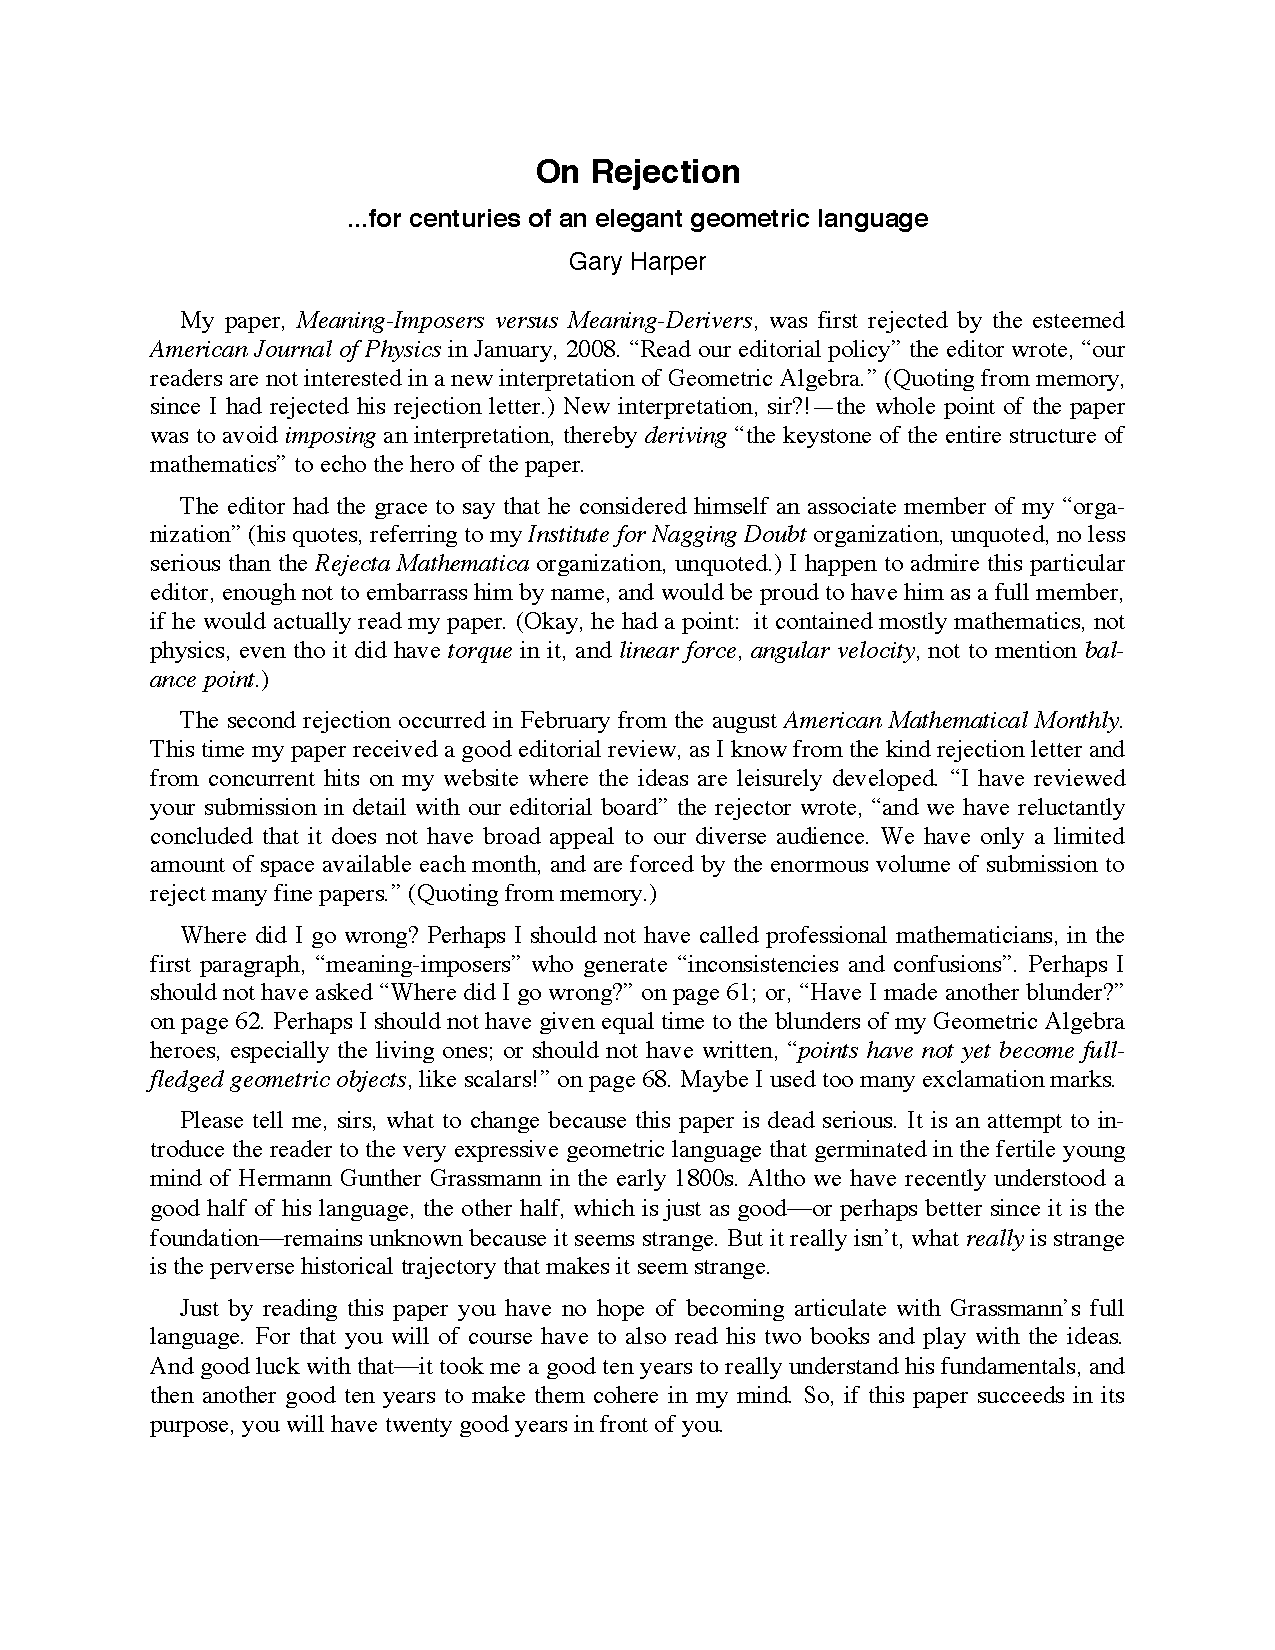
\includepdf[pages=-,pagecommand={\pagestyle{fancy}},noautoscale, scale=.9,offset={0pt -40pt}]{author_source/Schnass/openletter/openletter}
%\phantomsection
%\addcontentsline{toc}{subsection}{\textsf{\small{Paper}}}
\fancyhead{}
\fancyhead[L]{\small{{K. Schnass and P. Vandergheynst}}}
\fancyhead[R]{\small{\textit{\textsf{Classification via incoherent subspaces}}}}
\renewcommand{\headrulewidth}{0.4pt}
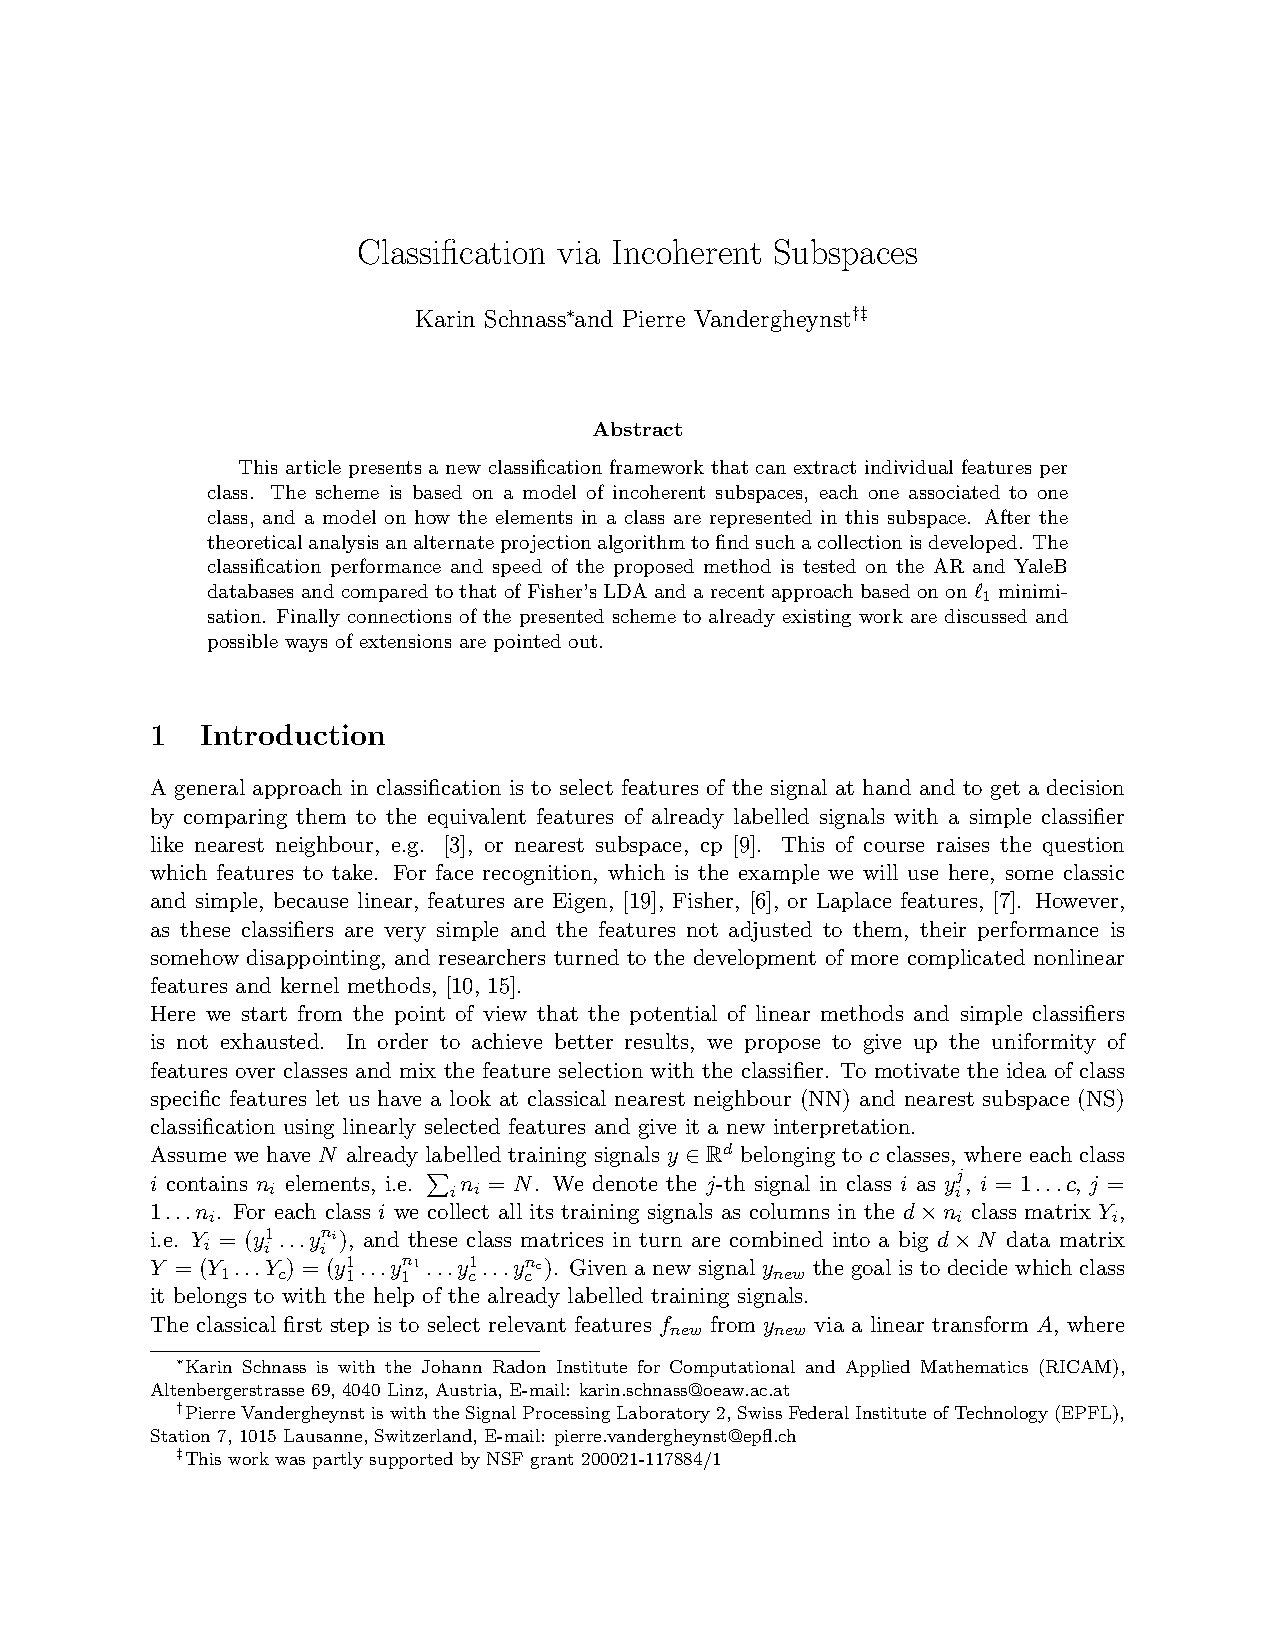
\includepdf[pages=-,pagecommand={\pagestyle{fancy}},noautoscale, scale=.9,offset={0pt -3pt}]{author_source/Schnass/article/Classification}


%Shanker
\phantomsection
\addcontentsline{toc}{section}{\small{\textsf{Explanation of low Hurst exponent for Riemann zeta zeros}}}
\addtocontents{toc}{
	\hbox{\textit{\footnotesize{\textsf{Oruganti Shanker}}}}
}
%\phantomsection
%\addcontentsline{toc}{subsection}{\textsf{\small{Open Letter}}}
\fancyhead{}
\fancyhead[L]{
	\includegraphics[width=.08\linewidth]{logoNotext}\vspace{.2cm}\\
	\large{\textit{\textsf{ARTICLE}}}
}
\fancyhead[R]{{\scriptsize{\textbf{
	Oruganti Shanker\\
	Explanation of low Hurst exponent for Riemann zeta zeros\\
	\emph{Rejecta Mathematica}, Vol. 2, No. 1, pp. 19--23, June 2011\\
	2011 Rejecta Publications\\
	\vspace{-.15cm}
	\href{http://math.rejecta.org}{math.rejecta.org}%
}}}}
\renewcommand{\headrulewidth}{0.4pt}
\includepdf[pages=-,pagecommand={\pagestyle{fancy}},noautoscale, scale=.9,offset={0pt -40pt}]{author_source/Shanker/openletter/openletter_Shanker}
%\phantomsection
%\addcontentsline{toc}{subsection}{\textsf{\small{Paper}}}
\fancyhead{}
\fancyhead[L]{\small{{O. Shanker}}}
\fancyhead[R]{\small{\textit{\textsf{Explanation of low Hurst exponent for Riemann zeta zeros}}}}
\renewcommand{\headrulewidth}{0.4pt}
\includepdf[pages=-,pagecommand={\pagestyle{fancy}},noautoscale, scale=.9,offset={0pt -3pt}]{author_source/Shanker/article/manuscript_Shanker}
\newpage





%Nayebi
\phantomsection
\addcontentsline{toc}{section}{\small{\textsf{On the distribution of Carmichael numbers}}}
\addtocontents{toc}{
	\hbox{\textit{\footnotesize{\textsf{Aran Nayebi}}}}
}
%\phantomsection
%\addcontentsline{toc}{subsection}{\textsf{\small{Open Letter}}}
\fancyhead{}
\fancyhead[L]{
	\includegraphics[width=.08\linewidth]{logoNotext}\vspace{.2cm}\\
	\large{\textit{\textsf{ARTICLE}}}
}
\fancyhead[R]{{\scriptsize{\textbf{
	Aran Nayebi\\
	On the distribution of Carmichael numbers\\
	\emph{Rejecta Mathematica}, Vol. 2, No. 1, pp. 24--43, June 2011\\
	2011 Rejecta Publications\\
	\vspace{-.15cm}
	\href{http://math.rejecta.org}{math.rejecta.org}%
}}}}
\renewcommand{\headrulewidth}{0.4pt}
\includepdf[pages=-,pagecommand={\pagestyle{fancy}},noautoscale, scale=.9,offset={0pt -40pt}]{author_source/Nayebi/openletter/nayebi_openletter}
%\phantomsection
%\addcontentsline{toc}{subsection}{\textsf{\small{Paper}}}
\fancyhead{}
\fancyhead[L]{\small{{A. Nayebi}}}
\fancyhead[R]{\small{\textit{\textsf{On the distribution of Carmichael numbers}}}}
\renewcommand{\headrulewidth}{0.4pt}
\includepdf[pages=-,pagecommand={\pagestyle{fancy}},noautoscale, scale=.9,offset={0pt -3pt}]{author_source/Nayebi/article/nayebi_manuscript}


%Shirali
\phantomsection
\addcontentsline{toc}{section}{\small{\textsf{Extended real number system in measure theory}}}
\addtocontents{toc}{
	\hbox{\textit{\footnotesize{\textsf{Satish Shirali}}}}
}
%\phantomsection
%\addcontentsline{toc}{subsection}{\textsf{\small{Open Letter}}}
\fancyhead{}
\fancyhead[L]{
	\includegraphics[width=.08\linewidth]{logoNotext}\vspace{.2cm}\\
	\large{\textit{\textsf{ARTICLE}}}
}
\fancyhead[R]{{\scriptsize{\textbf{
	Satish Shirali\\
	Extended real number system in measure theory\\
	\emph{Rejecta Mathematica}, Vol. 2, No. 1, pp. 44--48, June 2011\\
	2011 Rejecta Publications\\
	\vspace{-.15cm}
	\href{http://math.rejecta.org}{math.rejecta.org}%
}}}}
\renewcommand{\headrulewidth}{0.4pt}
\includepdf[pages=-,pagecommand={\pagestyle{fancy}},noautoscale, scale=.9,offset={0pt -40pt}]{author_source/Shirali/openletter/openletter_Shirali}
%\phantomsection
%\addcontentsline{toc}{subsection}{\textsf{\small{Paper}}}
\fancyhead{}
\fancyhead[L]{\small{{S. Shirali}}}
\fancyhead[R]{\small{\textit{\textsf{Extended real number system in measure theory}}}}
\renewcommand{\headrulewidth}{0.4pt}
\includepdf[pages=-,pagecommand={\pagestyle{fancy}},noautoscale, scale=.9,offset={0pt -3pt}]{author_source/Shirali/article/manuscript_Shirali}


%Bauer
\phantomsection
\addcontentsline{toc}{section}{\small{\textsf{The problematic nature of G\"{o}del's theorem}}}
\addtocontents{toc}{
	\hbox{\textit{\footnotesize{\textsf{Hermann Bauer and Christoph Bauer}}}}
}
%\phantomsection
%\addcontentsline{toc}{subsection}{\textsf{\small{Open Letter}}}
\fancyhead{}
\fancyhead[L]{
	\includegraphics[width=.08\linewidth]{logoNotext}\vspace{.2cm}\\
	\large{\textit{\textsf{ARTICLE}}}
}
\fancyhead[R]{{\scriptsize{\textbf{
	Hermann Bauer and Christoph Bauer\\
	The problematic nature of G\"{o}del's theorem\\
	\emph{Rejecta Mathematica}, Vol. 2, No. 1, pp. 49--58, June 2011\\
	2011 Rejecta Publications\\
	\vspace{-.15cm}
	\href{http://math.rejecta.org}{math.rejecta.org}%
}}}}
\renewcommand{\headrulewidth}{0.4pt}
\includepdf[pages=-,pagecommand={\pagestyle{fancy}},noautoscale, scale=.9,offset={0pt -40pt}]{author_source/Bauer/openletter/openletter_Bauer}
%\phantomsection
%\addcontentsline{toc}{subsection}{\textsf{\small{Paper}}}
\fancyhead{}
\fancyhead[L]{\small{{H. Bauer and C. Bauer}}}
\fancyhead[R]{\small{\textit{\textsf{The problematic nature of G\"{o}del's theorem}}}}
\renewcommand{\headrulewidth}{0.4pt}
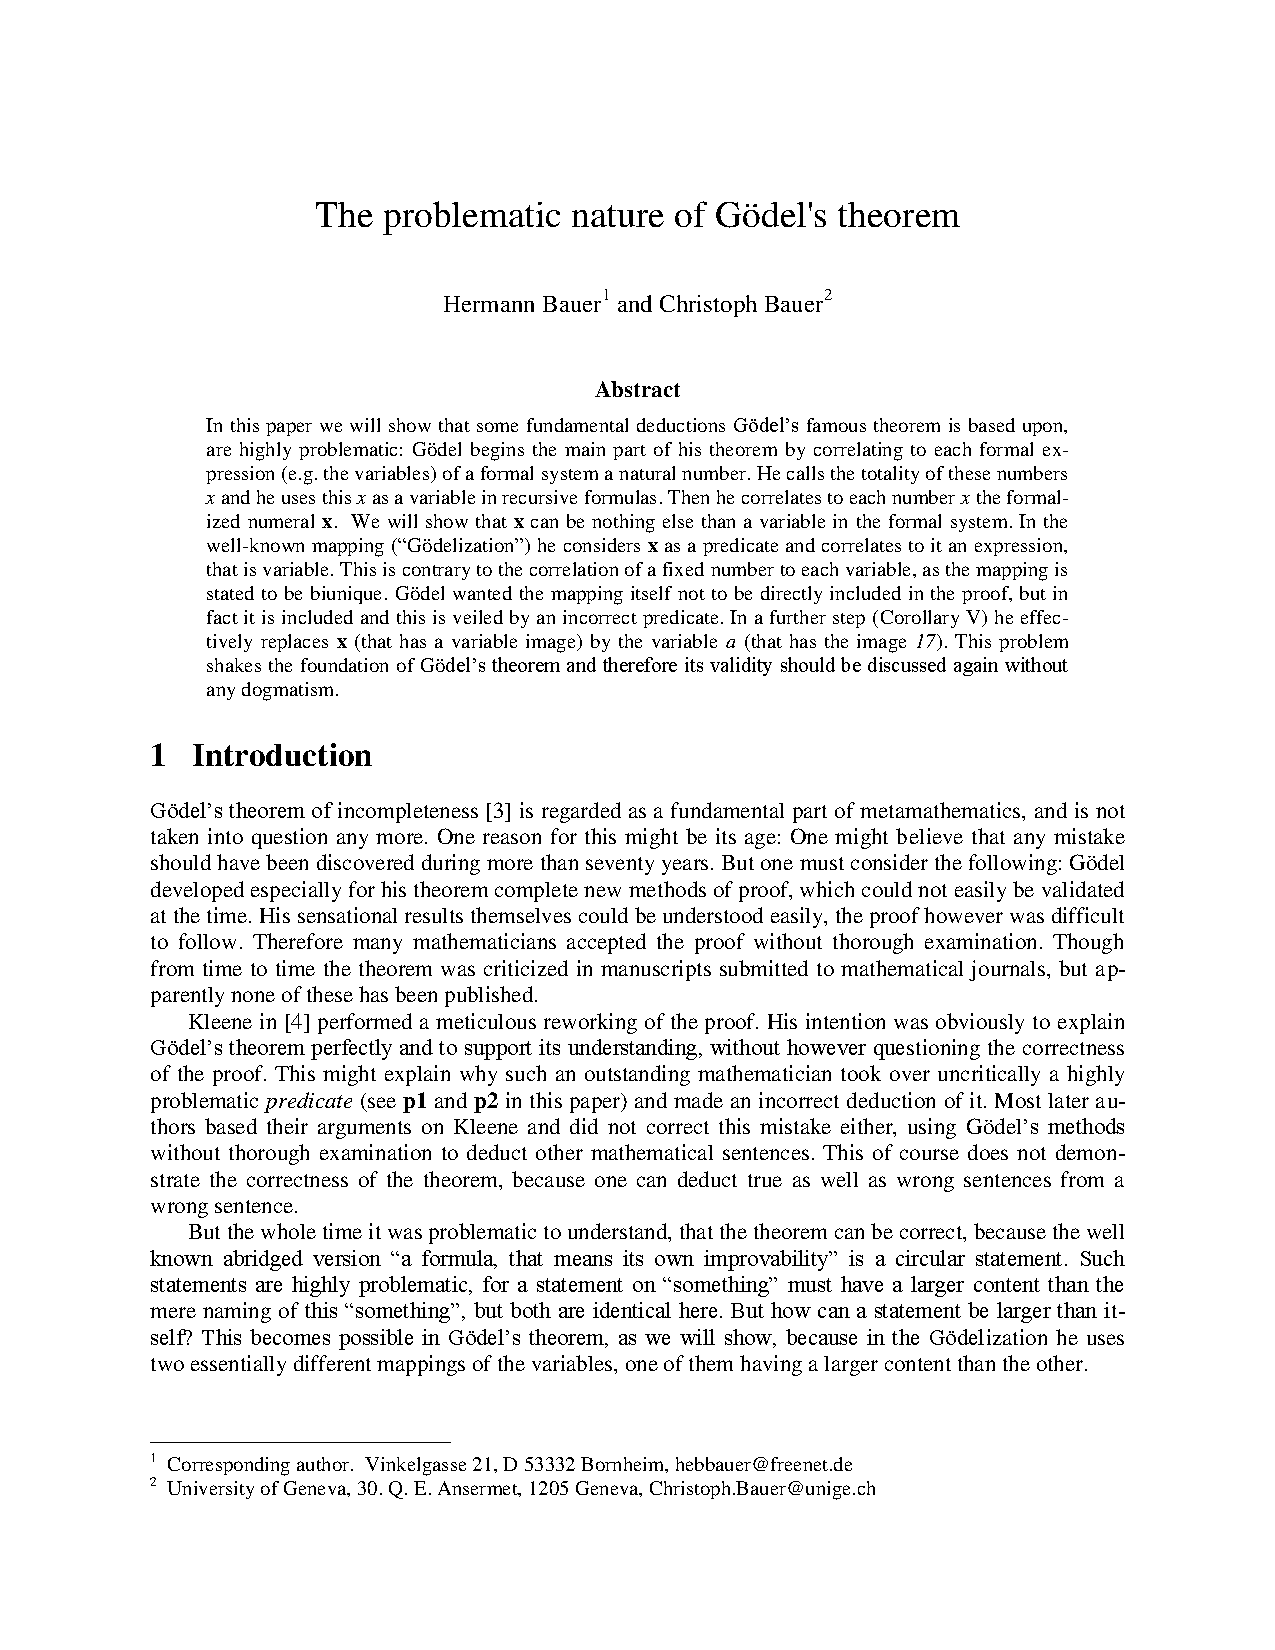
\includepdf[pages=-,pagecommand={\pagestyle{fancy}},noautoscale, scale=.9,offset={0pt -3pt}]{author_source/Bauer/article/manuscript_Bauer}
%\epageDZfalse

%Burnol
\phantomsection
\addcontentsline{toc}{section}{\small{\textsf{Scattering, determinants, hyperfunctions in relation to $\frac{\Gamma(1-s)}{\Gamma(s)}$}}}
\addtocontents{toc}{
	\hbox{\textit{\footnotesize{\textsf{Jean-Fran\c cois Burnol}}}}
}
%\phantomsection
%\addcontentsline{toc}{subsection}{\textsf{\small{Open Letter}}}
\fancyhead{}
\fancyhead[L]{
	\includegraphics[width=.08\linewidth]{logoNotext}\vspace{.2cm}\\
	\large{\textit{\textsf{ARTICLE}}}
}
\fancyhead[R]{{\scriptsize{\textbf{
	Jean-Fran\c cois Burnol\\
	Scattering, determinants, hyperfunctions in relation to $\frac{\Gamma(1-s)}{\Gamma(s)}$\\
	\emph{Rejecta Mathematica}, Vol. 2, No. 1, pp. 59--118, June 2011\\
	2011 Rejecta Publications\\
	\vspace{-.15cm}
	\href{http://math.rejecta.org}{math.rejecta.org}%
}}}}
\renewcommand{\headrulewidth}{0.4pt}
\includepdf[pages=-,pagecommand={\pagestyle{fancy}},noautoscale, scale=.9,offset={0pt -40pt}]{author_source/Burnol/openletter/openletter_Burnol}
%\phantomsection
%\addcontentsline{toc}{subsection}{\textsf{\small{Paper}}}
\fancyhead{}
\fancyhead[L]{\small{{J. Burnol}}}
\fancyhead[R]{\small{\textit{\textsf{Scattering, determinants, hyperfunctions in relation to $\frac{\Gamma(1-s)}{\Gamma(s)}$}}}}
\renewcommand{\headrulewidth}{0.4pt}
\includepdf[pages=-,pagecommand={\pagestyle{fancy}},noautoscale, scale=.9,offset={0pt -3pt}]{author_source/Burnol/article/manuscript_Burnol}
%\epageDZfalse







\end{document}  